\documentclass{article}
\usepackage[utf8]{inputenc}
\usepackage{mathtools}
\usepackage{enumerate}
\usepackage{pgfplots}
\usepackage{tikz}
\usepackage{amsthm}
\usepackage{amssymb}
\usepackage{float}
\usepackage{anysize}

\marginsize{2cm}{2cm}{2cm}{2cm}

\title{Sistemas expertos probabilísticos}
\author{Anabel Gómez Ríos\\
        Jacinto Carrasco Castillo}
\date{Mayo 2016}

% Definición de estilo de definición
\newtheoremstyle{definition_wo_parentheses}
  {\topsep}% measure of space to leave above the theorem. E.g.: 3pt
  {\topsep}% measure of space to leave below the theorem. E.g.: 3pt
  {}% name of font to use in the body of the theorem
  {0pt}% measure of space to indent
  {\bfseries}% name of head font
  {.}% punctuation between head and body
  { }% space after theorem head; " " = normal interword space
  {\thmname{#1}\thmnumber{ #2.}\thmnote{ #3}}
  
  
\theoremstyle{definition_wo_parentheses}	
\newtheorem{definicion}{Definición}

\begin{document}

\maketitle

\section{Introducción}
En clase hemos visto sistemas expertos basados en reglas del tipo \textbf{SI} \textit{condición} \textbf{ENTONCES} \textit{acción} (donde tanto en \textit{condición} como en \textit{acción} pueden aparecer expresiones lógicas compuestas). En estos sistemas se comprueba si \textit{condición} es cierta o no y, en caso de serlo, se lleva a cabo \textit{acción}.\\

Este tipo de sistemas son muy útiles y muy utilizados por su simplicidad y el parecido con el razonamiento humano, pero presentan varios inconvenientes:
\begin{enumerate}
    \item Mantener la coherencia entre las reglas de la base de conocimiento. Pueden aparecer dos tipos de problemas: encadenamientos infinitos, cuando aparecen reglas del tipo \textit{Si A entonces B} junto con \textit{Si B entonces A} y problemas de ampliación en la base de conocimiento cuando hay que realizar una actualización y para mantener la coherencia la base de datos se hace innecesariamente grande, llegando incluso a ser mejor reconstruirla de nuevo.
    \item Dificultades para retractarse de anteriores conclusiones, provocado principalmente por el carácter modular y monótono de estos sistemas, ya que cuando se cumple la condición de una regla, se da la acción sin tener en cuenta el resto del conocimiento.
    \item Opacidad: Al tener que dividir el conocimiento en pequeñas reglas, se pierde perspectiva global del problema tratado.
    \item Ineficiencia provocada por la continua comprobación de las reglas en cada iteración.
\end{enumerate}

Sin embargo el principal problema es que cuando se trabaja con problemas reales y conocimiento humano en la mayoría de los casos hay inherente incertidumbre bien en el conocimiento, es decir, en cómo se ha obtenido el conocimiento, o bien en el conjunto de datos, es decir, si los datos no se han determinado de forma precisa o faltan datos.\\
Normalmente, las evidencias que tenemos sobre un hecho no nos permiten deducir con seguridad las conclusiones o la negación de las mismas, pero sí nos permiten dar mayor credibilidad a una sentencia. Por esto, si queremos diseñar un sistema experto capaz de obtener las mismas conclusiones que un experto humano, tenemos darle la capacidad de trabajar con incertidumbre.

\section{Ejemplo de sistema experto Probabilístico: MYCIN}
MYCIN fue el primer sistema experto que consideró conocimiento incierto. En este sistema, una regla \textbf{Si} A \textbf{Entonces} B se representaba $A \overset{m}{\rightarrow}B$, expresando que si se conoce $A$, entonces se puede actualizar la certeza de $B$ en cierta cantidad, en función de la fuerza de la regla, $m$. El valor $m$ se denomina factor de certeza de la regla y toma valores en el intervalo $[-1,1]$.\\

Supongamos el siguiente ejemplo:
\[A \overset{m_1=0.8}{\longrightarrow} B ; B\ y\ C \overset{m_2=0.7}{\longrightarrow} D
\]
y observamos $A$ (y por tanto la certeza de $A$, que vamos a representar $Ctz(A)$ es 1) y la certeza sobre $C$ es 0.6. Entonces, nuestra creencia de $B$ se actualiza a un valor 0.8, $Ctz(B)=0.8$ y tenemos que actualizar la certeza sobre $D$. En estos casos, MYCIN calcula el valor de certeza para la sentencia $B\ y \ C$ como una función de las certezas de $A$ y $B$: $Ctz(B\ y\ C) = min{0.8,0.6}=0.6$ y por tanto $Ctz(D)=0.6*0.7=0.42$.\\
%?
Después veremos mecanismos de propagación que permiten trabajar con sistemas más complejos.

\section{Problemas de los sistemas expertos con incertidumbre}
\begin{enumerate}
    \item Aparecen problemas cuando tratamos de utilizar un razonamiento en los dos sentidos, ya que puede llevar a ciclos indefinidos (por ejemplo con las reglas \textit{\textbf{Si} hay humo \textbf{Entonces} es más creíble que haya fuego} y \textit{\textbf{Si} hay fuego \textbf{Entonces} hay humo}.
    \item No tratan de forma adecuada las fuentes de información dependientes, ya que cuando se dispara una regla, el peso que se asigna a la conclusión depende sólo del peso de las premisas, no de dónde vienen, y puede que vengan de una única fuente que ha seguido diferentes caminos o de fuentes independientes (esto debería influir en la certeza, ya que nos está llegando información de dos sitios distintos).
\end{enumerate}

\section{Comparación con los sistemas expertos basados en reglas}

\subsection{Base de conocimiento}

El conocimiento de un sistema experto basado en reglas consiste en los hechos y el conjunto de reglas. En un sistema experto basado en probabilidad, el conocimiento viene dado por un espacio de probabilidad que incluye las variables, sus posibles valores y su función de probabilidad conjunta. En ambos sistemas los datos consisten en la evidencia asociada a los casos a analizar.\\
Las diferencias también se encuentran en la dificultad para implementar la base de conocimientos. Mientras que en el sistema experto basado en reglas ``sólo'' necesitamos usar elementos como objetos, conjunto de valores, premisas, conclusiones y reglas; en los sistemas expertos basados en probabilidad el conocimiento puede ser mucho más extenso. Por contra, son necesarios numerosos parámetros, lo que dificulta su definición.

\subsection{Motor de inferencia}

El motor de inferencia también es más sencillo de implementar en los sistemas expertos basados en reglas, ya que obtenemos las conclusiones a partir de los hechos aplicando estrategias de inferencia como \textit{modus ponens}, \textit{modus tollens} y encadenamiento de reglas. En los sistemas expertos basados en probabilidad, el motor de inferencia se basa en la evaluación de las probabilidades condicionales, utilizando uno o varios métodos propuestos por diferentes tipos de sistemas expertos probabilísticos. El grado de dificultad de implementar un motor de inferencia probabilístico será mayor y crece si usamos modelos de dependencia generales en detrimento de modelos de independencia.

\subsection{Subsistema de explicación}

La explicación en el sistema basado en regla viene dada por las reglas que se han activado para determinar esa conclusión en cada momento. En el caso probabilístico la información sobre qué variables influyen en otras está codificada en la función de probabilidad conjunta, lo que hace que la explicación se base en los valores relativos de las probabilidades condicionales que miden los grados de dependencia. Una comparación de las probabilidades condicionales para diferentes conjuntos de evidencia permite analizar sus efectos en las conclusiones.

\subsection{Subsistema de aprendizaje}

En los sistemas expertos basados en reglas, el aprendizaje consiste en incorporar nuevos objetos, valores factibles para los objetos, nuevas reglas o modificaciones de los conjuntos existentes, valores posibles o reglase. En los sistemas expertos probabilísticos, consiste en incorporar o modificar la estructura del espacio de probabilidad: variables, posibles valores o parámetros.

\section{Teoría de la Probabilidad}
Vamos a ver algunas nociones básicas de probabilidad que serán de utilidad para trabajar con este tipo de sistemas.

\subsection{Probabilidad marginal}
Sean $X_1,X_2,...,X_n$ un conjunto de variables aleatorias que toman valores discretos y sea $\{x_1,x_2,...,x_n\}$ el conjunto de sus posibles realizaciones. Sea $P(x_1,x_2,...,x_n)$ una probabilidad sobre $X_1,X_2,...,X_n$, es decir, $P(x_1,x_2,...,x_n) = P(X_1 = x_1,...,X_n=x_n)$, entonces la distribución de probabilidad marginal sobre la $i$-ésima variables se obtiene mediante
\[	P(x_i) = P(X_i=x_i) = \sum_{x_1,...,x_{i-1},x_{i+1},...,x_n}P(x_1,...,x_n)	\]

\subsection{Probabilidad condicionada}
Sean $X$ e $Y$ dos conjuntos disjuntos de variables que toman valores en $\{x_1,...,x_n\}$ y $\{y_1,...,y_m\}$. La distribución de probabilidad condicionada de $X$ dado que $Y=y_j$ (con $j \in \{1,...,m\}$ y $P(Y=y_i)>0$) viene dada por
\[	\forall x_i \in X;\ P(X=x_i|Y=y_i)=P(x_i|y_i)=\frac{P(x_i,y_j)}{P(y_j)}	\]
Por tanto, la distribución de probabilidad conjunta puede obtenerse como:
\[	P(x_i,y_i)=P(y_j)P(x_i,y_j)	\]
La distribución de probabilidad conjunta nos va a permitir actualizar nuestro conocimiento a la luz de nueva información.

\subsection{Independencia probabilística}
Sean $X$ e $Y$ dos subconjuntos disjuntos del conjunto de variables aleatorias $\{X_1,...,X_n\}$. Se dice que $X$ es \textbf{marginalmente independiente} de $X$ y se nota $I(X,\emptyset,Y)$, si y solamente si para todos los posibles valores $x$ de $X$ e $y$ de $Y$ se satisface que $P(x|y)=P(x)$.\\
En caso contrario, se dice que $X$ es marginalmente dependiente de $Y$, y se denota $\neg I(X,\emptyset,Y)$.\\

Sean $X, Y$ y $Z$ tres conjuntos disjuntos de variables. Se dice que $X$ es \textbf{condicionalmente independiente} de $Y$ dado que conocemos $Z$, y lo notamos $I(X,Z,Y)$, si y sólo si para todos los valores $x,y,z$ de $X,Y,Z$ (respectivamente) se satisface que $P(x|z,y)=P(x|z)$.\\
En caso contrario se dice que son condicionalmente dependientes, y lo notamos por $\neg I(X,Z,Y)$.

\subsection{Teorema de Bayes}
Este teorema nos permite representar la probabilidad condicionada $P(y|x)$ mediante la expresión:
\[	P(y|x)=\frac{P(x|y)P(y)}{P(x)}	\]
Si tenemos en cuenta que $P(x) = \sum_{y \in Y}P(x,y)$ y que $P(x,y) = P(x|y)P(y)$ podemos reescribir la anterior expresión:
\[	P(x|y) = \frac{P(x|y)P(y)}{\sum_{y \in Y} P(x|y)P(y)}	\]

\section{Sistemas Expertos Probabilísticos}
Son dos los elementos esenciales que caracterizan a un sistema experto: La base de conocimiento y el motor de inferencia. Desde un punto de vista general, en un sistema experto probabilístico la base de conocimiento está formada por un conjunto de variables $X_1,...,X_n$ y una distribución de probabilidad conjunta sobre ellas $P(x_1,...,x_n)$. Por otro lado, un motor de inferencia básico sará aquel que nos permita actualizar nuestra información sobre una determinada variable (o conjunto de ellas), $X$, ante la presencia de un conjunto de hechos, evidencias o síntomas determinados, $E$. En teoría de la probabilidad este motor de inferencia no es más que el cálculo de la probabilidad condicional $P(X|E)$.\\
Si tratamos de realizar una aproximación directa, en la que representamos la distribución de probabilidad conjunta con una tabla, pronto nos damos cuenta de que, incluso en problemas con un conjunto pequeño de variables, el problema es intratable. Sin embargo, son muchas las aplicaciones prácticas en las que conocemos \textit{a priori} que, por ejemplo, dos variables son (marginal o condicionalmente) independientes. En estos casos, podemos utilizar dicha información con el objetivo de reducir el espacio necesario para almacenar la distribución de probabilidad conjunta. La idea es dividir o factorizar dicha distribución en un conjunto de distribuciones más pequeñas que tengan la misma representatividad. En cualquier caso, es necesario proporcionar un método que permita recuperar los valores originales de la distribución de probabilidad conjunta.\\
La idea básica es codificar el conocimiento de tal manera que no sea necesario el utilizar información que sea irrelevante y, por otro lado, la información relevante sea fácilmente accesible. Podemos encontrar distintos modelos para implementar esta idea, entre los que se encuentran las redes de Markov y las redes Bayesianas. Ambos sistemas se apoyan en modelos gráficos para representar de forma explícita las relaciones de dependencia e independencia entre las variables.

\section{Redes de Markov}
Las redes de Markov se representan gráficamente mediante grafos no dirigidos, donde los nodos representan las variables y una relación de dependencia entre dos variables se representa mediante la existencia de un camino o conexión entre ellas. Por otra parte, en estos modelos también se representan las relaciones de independencia. En concreto, si $X,Y$ y $Z$ son conjuntos disjuntos de variables, entonces:
\begin{enumerate}
\item Una independencia marginal viene representada por la inexistencia de conexión entre las variables de $X$ e $Y$.
\item Una relación de independencia condicionada del tipo $I(X,Z,Y)$ se representa por el hecho de que todo camino que conecta las variables de $X$ con variables de $Y$ contiene algún nodo de $Z$. Por tanto, si los nodos en $Z$ son borrados del grafo, las variables $X$ e $Y$ quedan desconectadas.\\
De esta forma, somos capaces de determinar cuándo dos variables son dependientes o no. Pero, ¿puede el modelo gráfico representar todas las relaciones de dependencia / independencia que se derivan de una distribución de probabilidad conjunta?\\
La respuesta a esta pregunta es que no. Supongamos el siguiente ejemplo:
\begin{figure}[H]
\centering
\includegraphics[width=0.3\textwidth]{ejemplo}
\caption{Ejemplo} \label{fig:ejemplo}
\end{figure}

De aquí podemos deducir varias cosas:
\begin{enumerate}
\item Como $P(x|y)=\frac{P(x,y)}{P(y)} = \frac{0.245+0.105}{0.03+0.12+0.245+0.105} = \frac{0.35}{0.5} = 0.7$ y $P(x)=0.21+0.14+0.245+0.105 = 0.7$ tenemos que $P(x|y)=P(x)$ y por tanto $X$ es independiente marginalmente a $Y \Rightarrow$ no exite un camino que conecte $X$ con $Y$.
\item De forma análoga se puede comprobar que $P(x|z)\neq P(x)$ y por tanto existe un camino que conecta $X$ y $Z$ e igualmente con $Z$ e $Y$
\end{enumerate}

Nos queda por tanto el siguiente grafo:
\begin{center}
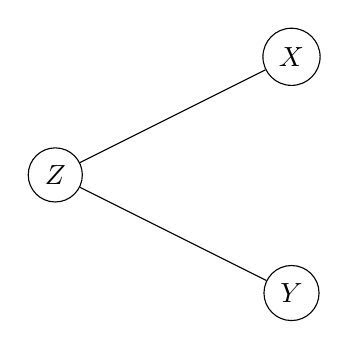
\begin{tikzpicture}[y=.3cm, x=.3cm,font=\normalsize]

\node[draw, circle] (X) at (10,10) {$X$};
\node[draw, circle] (Y) at (10,0) {$Y$};
\node[draw, circle] (Z) at (0,5) {$Z$};

\draw (X) -- (Z);
\draw (Z) -- (Y);

\end{tikzpicture}
\end{center}

De aquí podemos deducir que existe un camino que conecta $X$ con $Y$, el que pasa por $Z$, en contra de lo primera deducción. Las redes de Markov por tanto no son capaces de representar relaciones de independencia no transitivas. Una herramienta para diseñar sistemas expertos probabilísticos utilizando el formalismo más potente de los grafos dirigidos para representar las relaciones entre las variables son las redes bayesianas, que veremos a continuación.
\end{enumerate}

\section{Redes bayesianas}

\subsection{Conceptos previos}

Las redes bayesianas son uno de los modelos con más importancia en los sistemas expertos probabilísticos. Gráficamente consisten en un grafo dirigido acíclico, donde los nodos son variables del problema a resolver. Las redes bayesianas permiten representar dos aspectos del conocimiento:

\begin{enumerate}
\item \textbf{Cualitativo}: Relaciones de dependencia e independencia entre variables. Dos variables conectadas por un arco estarán relacionadas.
\item \textbf{Cuantitativo}: Fuerza con la que nos creemos las relaciones de relevancia o dependencia.
\end{enumerate}

Usaremos la representación mediante grafos para indicar la dependencia, por ejemplo, suponemos que representamos un problema que trata del alquiler de un vehículo para un viaje. Las variables son el \textit{Tipo de Vehículo}, \textit{Tipo de Carretera}, \textit{Velocidad Media} durante el viaje, \textit{Duración}, \textit{Precio} del alquiler y \textit{Kilómetros} a recorrer. Si hay un arco, habrá dependencia. 

\begin{center}
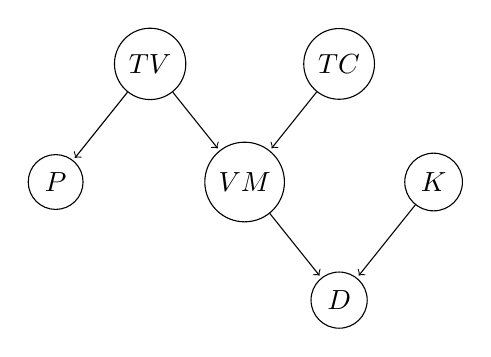
\begin{tikzpicture}[y=.3cm, x=.3cm,font=\normalsize,shorten >=1pt,->]

\node[draw, circle] (P) at (0,5) {$P$};
\node[draw, circle] (TV) at (4,10) {$TV$};
\node[draw, circle] (VM) at (8,5) {$VM$};
\node[draw, circle] (TC) at (12,10) {$TC$};
\node[draw, circle] (D) at (12,0) {$D$};
\node[draw, circle] (K) at (16,5) {$K$};

\draw (TV) -> (P);
\draw (TV) -> (VM);
\draw (VM) -> (D);
\draw (TC) -> (VM);
\draw (K) -> (D);

\end{tikzpicture}
\end{center}

Podemos decir que \textit{TC} y \textit{D} son variables dependientes, en cambio si conocemos \textit{VM} (velocidad media del viaje, \textit{TC} y \textit{D} son independientes. Esto induce el concepto de \textit{d-separación}.

\begin{definicion}[d-separación]
	Si $X,Y,Z$ son subconjuntos disjuntos de nodos en $G$ GDA (grafo dirigido acíclico), entonces $Z$ \textbf{d-separa} $X$ de $Y$ ($<X|Z|Y>_G$) si todos los caminos entre cualquier nodo de $X$ y cualquier nodo de $Y$ están bloqueados por $Z$. 
\end{definicion}

Esto nos permite representar las relaciones entre las variables. Ahora veremos cómo expresarlo de forma numérica. Supongamos dadas dos variables $X,Y$, $X \rightarrow Y$, debido a que hay una dependencia entre las dos variables. La incertidumbre asociada a este tipo de relaciones la podemos representar mediante el uso de una distribución de probabilidad condicionada sobre $Y$ dado $X$, $P(Y|X)$.\\
Cuando tenemos los valores para las distribuciones de probabilidad condicionadas, construimos la distribución de probabilidad conjunta sobre $X_1, \dots, X_n$:
\[ P(X_1, \dots,X_n) = \prod\limits_{i=1}^n P(X_i,\Pi(X_i))\]

donde $\Pi(X_i)$ representa el conjunto de padres de un nodo $X_i$ en la red.\\

Si relacionamos esto con el concepto de d-separabilidad visto anteriormente tenemos:

\begin{equation}
	<X|\emptyset|Y>_G \rightarrow P(X,Y) = P(X) P(Y)
\end{equation}
\begin{equation}
	<X|Y|Z>_G \rightarrow P(X|Y) = P(X|Y,Z)
\end{equation}

\subsection{Redes bayesianas y modelos de dependencia}



\section{Métodos de propagación}

%¿?
\section{Modelos en el campo de la medicina}

\section{Bibliografía}


\end{document}